\section{Introduction}
\label{sec:intro}

	La sécurisation des systèmes est l'une des problématiques majeures de la société moderne. En ce sens, de nombreuses méthodologies ont été développées dans le but d'identifier les risques et de les quantifier. C'est ainsi que le concept d'ADTrees\footnote{Abréviation d'\og Attack-Defense Trees \fg{}, ou \og Arbres d'Attaque et de Défense\fg{} en français.}, un formalisme permettant de représenter sous forme d'arbre les étapes d'une attaque précise contre un système, a vu le jour. L'un des logiciels destinés à leur modélisation informatique s'appelle ADTool.

    Lors de la prise en main de ce logiciel, nous avons trouvé qu'il présentait quelques limitations. Tout d'abord, ADTool ne fournissait pas d'outils permettant à l'utilisateur de simplifier l'analyse des ADTrees. En effet, dans un cas concret d'expertise en sécurité, l'ADTree utilisé sera parfois de très grande taille et dans ce cas, il est difficile pour l'expert d'en extraire des informations pertinentes au premier coup d’œil. Ensuite, il manquait à ADTool certaines fonctionnalités \og basiques \fg{} telles que le copier/coller ou l'annulation d'une action. 

    L'objectif de ce projet était la réalisation d'un logiciel permettant de dépasser ces limites en fournissant à l'utilisateur, un expert en sécurité, des outils d'analyse des ADTrees. Ce logiciel a été nommé \glasir{} en référence à l'arbre aux feuilles d'or de la mythologie nordique~\cite{vikingCulture}, et son logo est visible sur la \textsc{Figure} \ref{fig:glasir}. Il dispose de trois fonctionnalités principales qui ont été détaillées dans les rapports précédents : l'Éditeur de fonctions, le Filtre, et l'Optimiseur. ADTool a quant à lui été amélioré, et utilisé au sein de Glasir comme viewer d'ADTrees.

    Ce rapport a pour but de revenir sur les phases de planification et d'organisation du projet, au vu de son implémentation réelle. Dans un premier temps, il rappellera les principales lignes de la planification initialement prévue. Ensuite, il détaillera et justifiera les écarts à cette planification, constatés à la fin du développement effectif du logiciel. Une rétrospective concluera ce rapport, afin de proposer quelques pistes à suivre pour améliorer la gestion de nos projets à venir.

    \begin{figure}[h!]
        \centering
        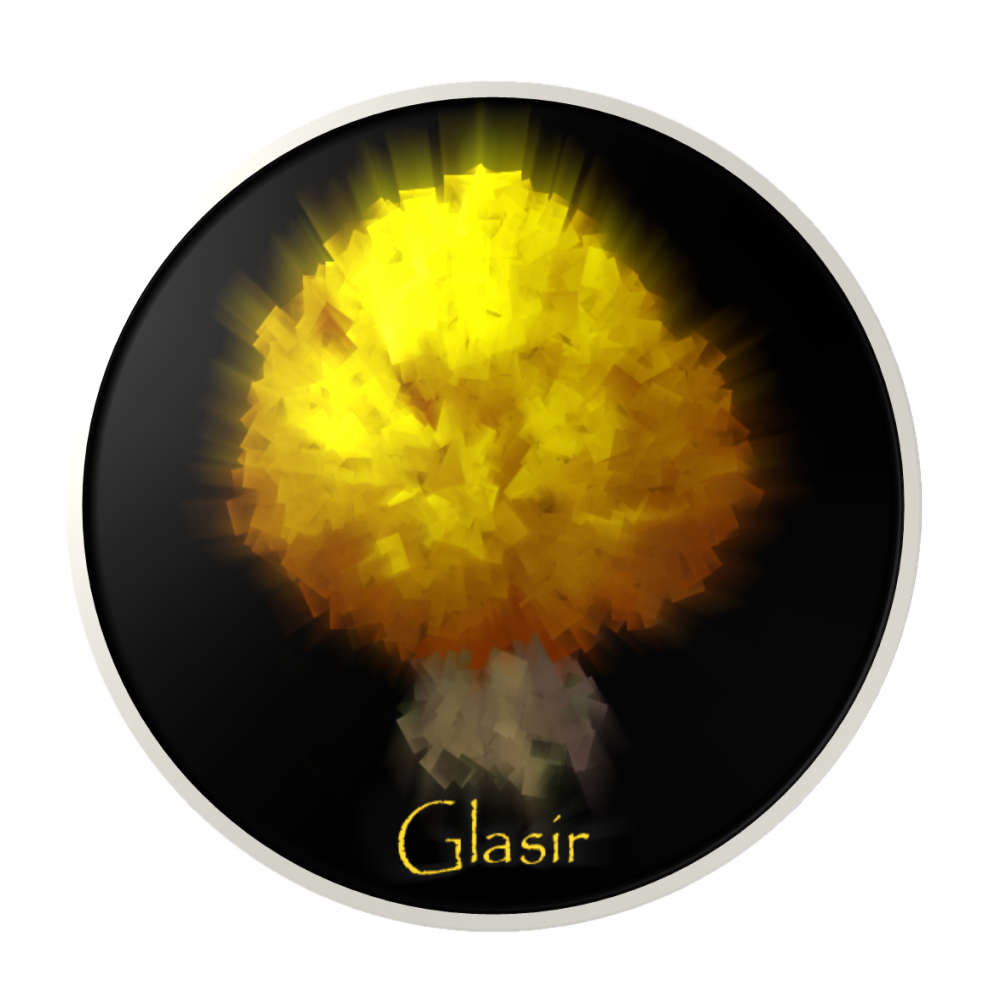
\includegraphics[height=0.4\textwidth]{figure/glasir.png}
        \caption{Logo du logiciel \glasir{}.}
        \label{fig:glasir}
    \end{figure}